\documentclass[letterpaper]{article}
\usepackage{aaai}
\usepackage{times}
\usepackage{helvet}
\usepackage{courier}
\usepackage{pgfplots}
\usepackage{amsmath}

 \pgfplotsset{compat=newest}
\frenchspacing
\setlength{\pdfpagewidth}{8.5in}
\setlength{\pdfpageheight}{11in}
\pdfinfo{
/Title (Acceleration of Fused Operations)
/Author (Andreas Falkenberg)}
\setcounter{secnumdepth}{0}  
 \begin{document}
\title{Acceleration of CUDA Kernels through Fusion \\ Measurements for AvgPool2D and Gelu}
\author{Andreas Falkenberg\\
Dr Falkenberg Technology Consulting Inc\\
366 Somerset Hills Glen\\
Escondido, California 92026\\
}

\maketitle

\begin{abstract}
\begin{quote}
The need to accelerate LLM (large language models) requires the use of always advancing compiler technologies. Operator fusion is one of the promising techniques to considerably improve the throughput of LLMs. This paper discusses the impact of operator fusion on the direct operator performans. The paper compares throughputs between pure CPU implementation, versus two kernel implementations versus a fused single kernel solution.  

\end{quote}
\end{abstract}

\noindent

One advanced optimization step in the development process of large language models (LLM) is the use of fused operators. Operator fusion is one of the techniques, which allow a considerable improvement of the throughput of an LLM running on accelerator hardware. It targets the shortcomings of using accelerators, which require to upload and download the data between each operation. This process is considerably shortend by the use of operator fusion. This paper specifically provides some measurements of the direct improvement of operator fusion by comparing operator performance with and without fusion being applied. In the paper the results of AvgPool2D operator fused with the Gelu operator is presented.


\section{Introduction}

In recent years the push for and the growth of Large Language Models (LLM) provided new challenges for processor and compiler developers to improve the throughput and performance of such models. The main challenge is to stay within the constraints of already existing hardware. Although hardware accelerators enter the market in relative rapid succession, companies may not be willing to upgrade their compute ressources with each new generation of processors and accelerators. Usually a software upgrade and tool upgrade is much more common and easier to achieve compared to an actual hardware upgrade.  
Essentially there are two areas, which are targeted to improve performance of LLMs. First there is the improvement of the hardware by utilizing new hardware architectures and improving existing hardware architectures by adding specific features, which benefit the processing of neural network workloads. The other area is the improvement by software tools. Specifically AI compilers are under development, which boost the performance of exising hardware by utilizing the specific AI accelerating features. \shortcite{7783725} \shortcite{10.1145/3520142} \shortcite{9443851} They also need to adapt quickly to support new features of new hardware. These optimizations are often in the area of parallel execution of workloads, faster data transfer between nodes and faster loading of kernels into the hardware to name a few. 
One newer optimization technique is the fusion of multiple neural network nodes into one single node. Thereby a set of operators are identified as fuseable, combined into one operator and finally mapped to the appropriate fused kernel. This paper discusses fusion of a AvgPool2D \shortcite {wang2021bambalancedattentionmechanism} operator with a Gelu operator. \shortcite{boehm2018optimizingoperatorfusionplans} The following sections provide a brief discussion of the underlying idea, then discuss some of the implementation and test features and environment. Lastly measured results are presented and a conclusion is given. 

\section{Motivation} 

A neural network workload constitutes of many nodes which mostly are executed individually or in eager mode. Eager mode means even with accelerating hardware, each node is executed on an individual basis and therefore the data is loaded in and out of the accelerator after each operation. A huge amount of data may be loaded to the accelerator, which then in a very aggressive highly parallel effort, performs such an operation quickly utilizing the parallel feature of the hardware accelerator and then load the result of said operation back to the host processor. A second node is processed in the exact same way, which means that the same or maybe a reduced or enlarged amount of data is loaded into the accelerator and the appropriate process is performed again. The neverthless means that data which might as well be processed within the same hardware is uploaded and downloaded between processing steps albeit being already at the correct location or stored in the correct memory.  
By fusing nodes the additional upload and download step of interim results are removed and the appropriate steps are directly performed. This usually leads to a considerable improvement in throughput and performance of the exact same model. We can see this specifically in the combination of matrix multiplication with immediately following activation functions. The optimization of matrix multiplication and its fusion with activation functions seems to be already widely discussed \shortcite{Acharya_2020}, \shortcite{li2023deepmodelfusionsurvey}. What is also mentioned in many publications is the overall impact on existing models, whereas there is little to no discussion about the impact of the individual contributing node, which would be an utmost important tool for developers of original neural network architectures. In this paper we discuss one specific combination of operations, which are very common in the context of Large Language Models. The first is the avgPool2D function and the second is the gelu function. Other publications will follow to discuss other combinations of operations. 

\section{The Approach}
Different solutions were executed to compare the runtime of a AvgPool2D operator and a Gelu operator between CPU and CUDA solutions. A small model with one AvgPool2D operator and one Gelu operator with flexible shapes is implemented in C++ to run on a CPU. Then a total of three kernels are developed in CUDA. The first kernel represents the AvgPool2d operation, the second kernel represents the Gelu operator and the third kernel represents the fused kernel, which constitutes of the said AvgPool2D operator directly followed by tbe Gelu operator implemented in one CUDA kernel. 

\subsection{AvgPool2D kernel implementation}
The implementation of the AvgPool2D kernel is based on the mathematical representation shown in equation~\ref{eq::avgPoolEq}:

\begin{equation}
\begin{aligned}
\label{eq::avgPoolEq} 
avgPool2D(N_i, C_j, h, w)  =  \frac{1}{kH * kW}  \sum_{m=0}^{kH-1} \sum_{n=0}^{kW-1} \\
                               input(N_i, C_j, stride[0] \times h + m, stride[1] \times w + n)
\end{aligned}
\end{equation}


The kernel is implemented in CUDA. The inner two loops are implemented on each of the nodes, which therefore would perform \(kH *kW\) operations each. The outer loops are mapped to the nodes of the CUDA hardware.  

\subsection{Gelu kernel implementation}

The gelu kernel is based on the mathematical definition in equation~\ref{eq::geluEq}:  

\begin{equation}
\label{eq::geluEq} 
GELU(x) = 0.5 * x * (1 + \tanh(\sqrt{2 / \pi} * (x + 0.044715 * x^3)))
\end{equation}



Each kernel performs the above Gelu operation, therefore mulitple of these operations can be mapped onto the CUDA platform to be executed in parallel. For this specific exercise there is no further optimization performed and the original Gelu function is used as in Figure~\ref{geluFunc}. Nevertheless it is recognized that there are proposals to improve the Gelu operation considerably by using partial functions with linear approximations. 

\begin{figure}
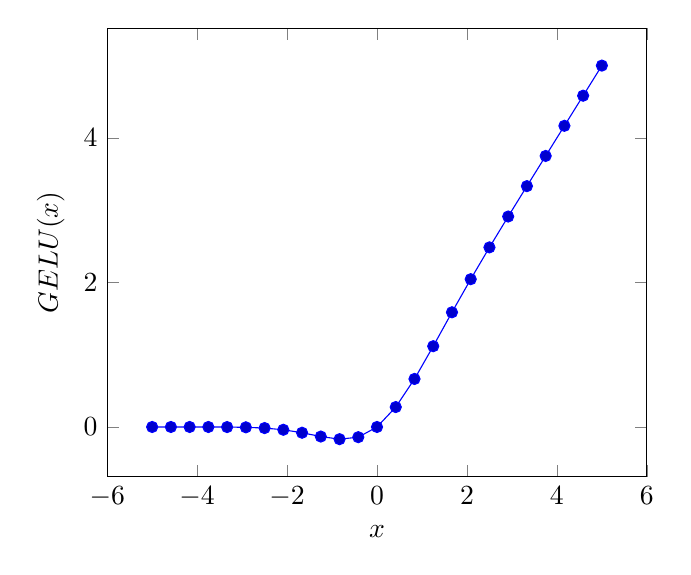
\begin{tikzpicture}
  \begin{axis}[ 
    xlabel=$x$,
    ylabel={$GELU(x)$}
  ] 
    \addplot {0.5 * x * (1 + tanh(sqrt(2/pi) * (x +0.044715 * x*x*x))) }; 
  \end{axis}
\end{tikzpicture}
\caption{GELU function}
\label{geluFunc}
\end{figure}

In the following sections the results are measured and presented. 

\section{Results}

In this section we show the results when running the individual kernels on CPU, then we show the combined solution running on CPU. Further we show the performance of the two CUDA kernels running back to back on a CUDA platform, and finally compare that with the fused kernel solution, which shows the real benefit of performing fusion in the first place. 

\subsection{CPU implementation of AvgPool2D}

The first result is based on a CPU implementation of AvgPool2D in C++ on a PC. In Figure~\ref{cpuAvgPool} we can clearly identify a linear behaviour based on the number of input elements. The kernel size as well as the stride size are set to eight for each dimension.  

\begin{figure}
\begin{tikzpicture}
\begin{axis}[
    xlabel={$dx$},
    ylabel={$sec$},
    legend entries={$dy=512$,$dy=1024$,$dy=1536$,$dy=2048$,$dy=2560$, $dy=3072$},
    legend pos=north west,
]
    \addplot [red] table {cpu_avgPool_dimi_512.dat};
    \addplot [blue] table {cpu_avgPool_dimi_1024.dat};
    \addplot [green] table {cpu_avgPool_dimi_1536.dat};
    \addplot [orange] table {cpu_avgPool_dimi_2048.dat};
    \addplot [magenta] table {cpu_avgPool_dimi_2560.dat};
    \addplot [yellow] table {cpu_avgPool_dimi_3072.dat};

\end{axis}
\end{tikzpicture}
\caption{AvgPool2D on CPU}
\label{cpuAvgPool}
\end{figure}

\subsection{AvgPool2D in sequence with Gelu on CPU}

The next implementation combines the AvgPool2D algorithm with Gelu. Since it is performed on the CPU we do not need to make a difference between the sequential and the parallel execution as well as the combined execution of the two operators. 

\begin{figure}
\begin{tikzpicture}
\begin{axis}[
    xlabel={$dx$},
    ylabel={$sec$},
    legend entries={$dy=512$,$dy=1024$,$dy=1536$,$dy=2048$,$dy=2560$, $dy=3072$},
    legend pos=north west,
]
    \addplot [red] table {cpu_avgPoolGelu_dimi_512.dat};
    \addplot [blue] table {cpu_avgPoolGelu_dimi_1024.dat};
    \addplot [green] table {cpu_avgPoolGelu_dimi_1536.dat};
    \addplot [orange] table {cpu_avgPoolGelu_dimi_2048.dat};
    \addplot [magenta] table {cpu_avgPoolGelu_dimi_2560.dat};
    \addplot [yellow] table {cpu_avgPoolGelu_dimi_3072.dat};

\end{axis}
\end{tikzpicture}
\caption{AvgPool2D with Gelu on CPU}
\label{cpuAvgPoolGelu}
\end{figure}

The Figure~\ref{cpuAvgPoolGelu} shows the result for AvgPool2D with Gelu in sequence. The inclusion of Gelu hardly contributes to the overall result on CPU. 

In Figure~\ref{cpuWithWithout} a direct comparisong of AvgPool2D without and with Gelu is shown. It is recognized that exercising Gelu on a CPU does not significantly change the overall runtime. The main explanation is that there is no additional allocation of memory involved since Gelu directly writes back to the same element. Further the number of elements is reduced now by 64, because the avgPool2D operation uses a 8x8 inner dimensions for our example.

\begin{figure}
\begin{tikzpicture}
\begin{axis}[
    xlabel={$dx$},
    ylabel={$sec$},
    legend entries={$only avgpool$, $with gelu$},
    legend pos=north west,
]
    \addplot [red] table {cpu_avgPool_dimi_3072.dat};
    \addplot [blue] table {cpu_avgPoolGelu_dimi_3072.dat};

\end{axis}
\end{tikzpicture}
\caption{AvgPool2D with/without Gelu on CPU}
\label{cpuWithWithout}
\end{figure}

\subsection{Performance of AvgPool2D kernel on CUDA} 

In the following subsections the CUDA results are presented. The first results as shown in Figure~\ref{cudaAvgPool} are based on the AvgPool2D cuda kernel. It shows that the parallel execution leads to almost no difference between smaller and larger workloads. The presented workloads are still small and therefore the major impact comes from the overhead of engaging with the GPU in the first place. Nevertheless the results clearly show that the CUDA implementation has a huge impact on the performance. 

\begin{figure}

\begin{tikzpicture}
\begin{axis}[
    xlabel={$dx$},
    ylabel={$sec$},
    legend entries={$dy=512$,$dy=1024$,$dy=1536$,$dy=2048$,$dy=2560$, $dy=3072$},
    legend pos=north east,
]
    \addplot [red] table {cuda_avgPool_dimi_512.dat};
    \addplot [blue] table {cuda_avgPool_dimi_1024.dat};
    \addplot [green] table {cuda_avgPool_dimi_1536.dat};
    \addplot [orange] table {cuda_avgPool_dimi_2048.dat};
    \addplot [magenta] table {cuda_avgPool_dimi_2560.dat};
    \addplot [yellow] table {cuda_avgPool_dimi_3072.dat};

\end{axis}
\end{tikzpicture}
\caption{AvgPool2D on CUDA}
\label{cudaAvgPool}
\end{figure}

\subsection{Performanace of Gelu kernel on CUDA}

If we only run the Gelu kernel Figure~\ref{cudaGelu} shows that for most cases the overhead to engage with the GPU has a higher impact than performing Gelu directly on the CPU. Nevertheless part of it is misleading since on the CPU we do not count the impact of the memory allocation, which is already done as part of the AvgPool2D output matrix memory allocation. 

\begin{figure}
\begin{tikzpicture}
\begin{axis}[
    xlabel={$dx$},
    ylabel={$sec$},
    legend entries={$dy=512$,$dy=1024$,$dy=1536$,$dy=2048$,$dy=2560$, $dy=3072$},
    legend pos=north east,
]
    \addplot [red] table {cuda_Gelu_dimi_512.dat};
    \addplot [blue] table {cuda_Gelu_dimi_1024.dat};
    \addplot [green] table {cuda_Gelu_dimi_1536.dat};
    \addplot [orange] table {cuda_Gelu_dimi_2048.dat};
    \addplot [magenta] table {cuda_Gelu_dimi_2560.dat};
    \addplot [yellow] table {cuda_Gelu_dimi_3072.dat};

\end{axis}
\end{tikzpicture}
\caption{Gelu on CUDA}
\label{cudaGelu}
\end{figure}

\subsection{AvgPool2D and Gelu in sequence}

To provide some better datapoints Figure~\ref{cudaAvgPoolGeluSeq} shows running the avgPool2D and the Gelu back to back, yet using separate kernels. We can clearly also see that there is some overhead compared to the prior solution. 

\begin{figure}
\begin{tikzpicture}
\begin{axis}[
    xlabel={$dx$},
    ylabel={$sec$},
    legend entries={$dy=512$,$dy=1024$,$dy=1536$,$dy=2048$,$dy=2560$, $dy=3072$},
    legend pos=north east,
]
    \addplot [red] table {cuda_avgPoolGelu_notMerged_512.dat};
    \addplot [blue] table {cuda_avgPoolGelu_notMerged_1024.dat};
    \addplot [green] table {cuda_avgPoolGelu_notMerged_1536.dat};
    \addplot [orange] table {cuda_avgPoolGelu_notMerged_2048.dat};
    \addplot [magenta] table {cuda_avgPoolGelu_notMerged_2560.dat};
    \addplot [yellow] table {cuda_avgPoolGelu_notMerged_3072.dat};

\end{axis}
\end{tikzpicture}
\caption{AvgPool2D and Gelu sequential on CUDA}
\label{cudaAvgPoolGeluSeq}
\end{figure}


The best result is achieved by using the fused kernel. The fused kernel incorporates avgPool2D and Gelu in one kernel and therefore the output of the avgPool2D is directly processed. The first result does not need to be copied to the main mamory and back to the kernel memory of the Gelu kernel any more. This allows to shave off a significant portion of the runtime and improve the performance significantly. 

\begin{figure}

\begin{tikzpicture}
\begin{axis}[
    xlabel={$dx$},
    ylabel={$sec$},
    legend entries={$dy=512$,$dy=1024$,$dy=1536$,$dy=2048$,$dy=2560$, $dy=3072$},
    legend pos=north east,
]
    \addplot [red] table {cuda_avgPoolGelu_merged_512.dat};
    \addplot [blue] table {cuda_avgPoolGelu_merged_1024.dat};
    \addplot [green] table {cuda_avgPoolGelu_merged_1536.dat};
    \addplot [orange] table {cuda_avgPoolGelu_merged_2048.dat};
    \addplot [magenta] table {cuda_avgPoolGelu_merged_2560.dat};
    \addplot [yellow] table {cuda_avgPoolGelu_merged_3072.dat};

\end{axis}
\end{tikzpicture}
\caption{AvgPool2D and Gelu fused on CUDA}
\label{cudaAvgPoolGeluFused}
\end{figure}




\section{Conclusion}

We conclude that kernel fusion has a significant impact on the performance and the throughput of a model. Although the fused kernel was not integrated into a realistic LLM workload this initial research already shows significant progress. The final figure combines the most significant results. We can see that only when a small matrix is used, i.e. at or below 128x3096, the CPU solution may be faster. 

\begin{figure}
\begin{tikzpicture}
\begin{axis}[
    xlabel={$dx$},
    ylabel={$sec$},
    legend entries={$CPU$, $CUDA$,$CUDA fused$},
    legend pos=north west,
]
    \addplot [red] table {cpu_avgPoolGelu_dimi_3072.dat};
    \addplot [blue] table {cuda_avgPoolGelu_notMerged_3072.dat};
    \addplot [green] table {cuda_avgPoolGelu_merged_3072.dat};

\end{axis}
\end{tikzpicture}
\caption{CPU vs CUDA vs fused CUDA}
\label{cudaGelu}
\end{figure}


The herein presented results are based on the implementation of a new CUDA based library, which concentrates solely on fused kernels for AI workloads. The progress of this work can be followed at \shortcite{falkenberg2024AvgPoolGelu}


\bibliography{AvgPoolGeluBib}
\bibliographystyle{aaai}

 
\end{document}
